%%%%%%%%%%%%%% ЗАДАНИЕ №1 %%%%%%%%%%%%%%
%% Условие задания №1
\begin{problem}
    
    М=\{33, 97, 69, 71, 42, 49, 51, 59\}\newline
	Бинарное отношение задано выражением: \newline
   $$ F_{1}(x,y)=1\Leftrightarrow\newline$$
 \newline
 Проверить, является ли бинарное отношение (далее -- б.о.) -- рефлексивным, арефлексивным, симметричным, антисимметричным, асимметричным, транзитивным.
\end{problem}

%% Решение задания №1
\begin{proof}
    Для удобства расположим числа, входящие в мн-во М в порядке возрастания и построим матрицу для данного бинарного отношения:
	$$ \left( \begin{array}{c c c c c c c c } 
 
 1 & 0 & 1 & 1 & 1 & 1 & 1 & 1 \\ 

 0 & 1 & 0 & 0 & 0 & 0 & 0 & 0 \\

 1 & 0 & 1 & 1 & 1 & 1 & 1 & 1 \\ 
 
 1 & 0 & 1 & 1 & 1 & 1 & 1 & 1 \\ 
 
 1 & 0 & 1 & 1 & 1 & 1 & 1 & 1 \\ 
 
 1 & 0 & 1 & 1 & 1 & 1 & 1 & 1 \\ 
 
 1 & 0 & 1 & 1 & 1 & 1 & 1 & 1 \\ 
 
 1 & 0 & 1 & 1 & 1 & 1 & 1 & 1  \end {array} \right) $$
 Б.о. рефлексивно, тк на главной диагонали матрицы все 1.
    \newline
     Б.о. симметрично, тк матрица симметрична относительно главной диагонали.
    \newline
    Б.о. транзитивно, тк при возведении матрицы в квадрат не появляются новые связи.
     \newline

\end{proof}

%%%%%%%%%%%%%% ЗАДАНИЕ №2 %%%%%%%%%%%%%%
%% Условие задания №2
\begin{problem}
	Постройте матрицу и граф этого б.о.
\end{problem}

%% Решение задания №2
\begin{proof}
Перед построением матрицы отсортируем вершины по возрастанию. Таким образом строчке(столбцу) с меньшим порядковым номером соответсвует вершина с меньшим значением, а строчке(столбцу) с большим порядковым номером -- вершина с большим значением.
	$$ \left( \begin{array}{c c c c c c c c } 
 
 1 & 0 & 1 & 1 & 1 & 1 & 1 & 1 \\ 

 0 & 1 & 0 & 0 & 0 & 0 & 0 & 0 \\

 1 & 0 & 1 & 1 & 1 & 1 & 1 & 1 \\ 
 
 1 & 0 & 1 & 1 & 1 & 1 & 1 & 1 \\ 
 
 1 & 0 & 1 & 1 & 1 & 1 & 1 & 1 \\ 
 
 1 & 0 & 1 & 1 & 1 & 1 & 1 & 1 \\ 
 
 1 & 0 & 1 & 1 & 1 & 1 & 1 & 1 \\ 
 
 1 & 0 & 1 & 1 & 1 & 1 & 1 & 1  \end {array} \right) $$
 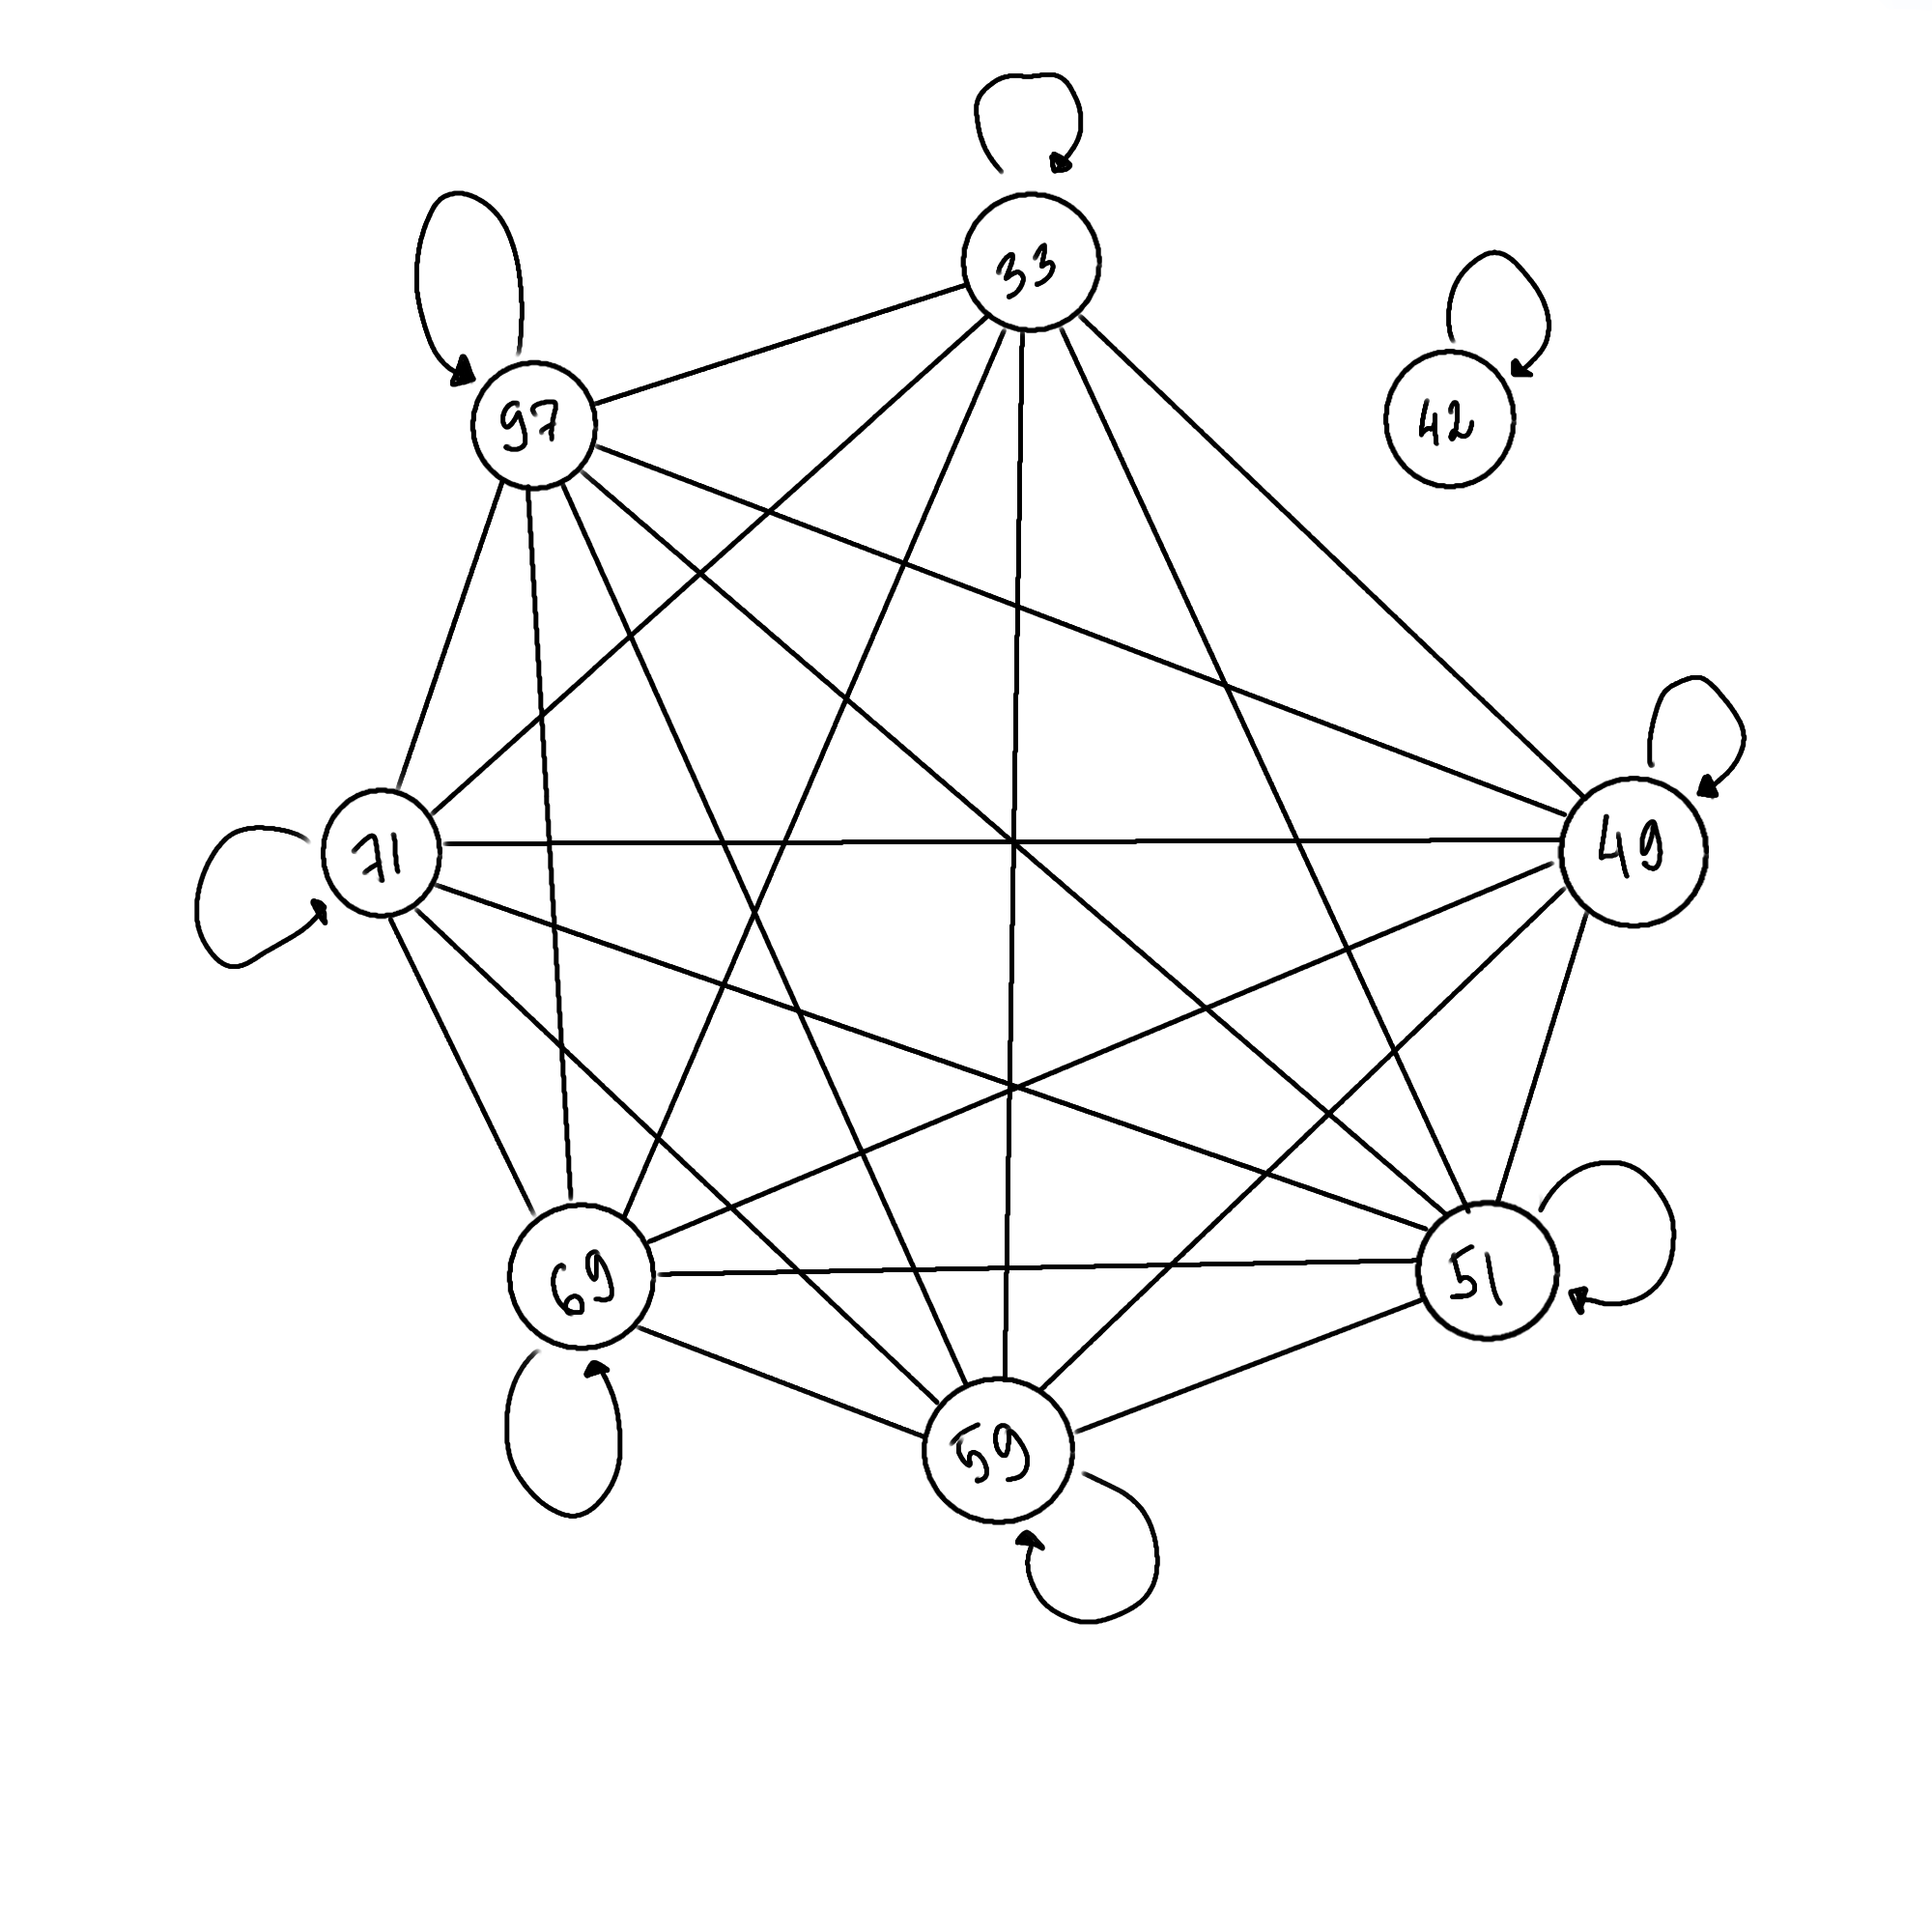
\includegraphics{граф4.png}
\end{proof}

%%%%%%%%%%%%%% ЗАДАНИЕ №3 %%%%%%%%%%%%%%
%% Условие задания №3
\begin{problem}
	Определить, является ли это б.о. отношением эквивалентности, частичного порядка, линейного порядка, строгого порядка.
\end{problem}

%% Решение задания №3
\begin{proof}
	Б. о. является отношением эквиваллентности, тк рефлексивно, симметрично и транзитивно.
\end{proof}
%%%%%%%%%%%%%% ЗАДАНИЕ №4 %%%%%%%%%%%%%%
%% Условие задания №4
\begin{problem}
	Для отношений эквивалентности построить классы эквивалентности.
\end{problem}

%% Решение задания №4
\begin{proof}
\{ 33, 49, 51, 59, 69, 71, 97\}\{ 42\}
\end{proof}
%%%%%%%%%%%%%% ЗАДАНИЕ №5 %%%%%%%%%%%%%%
%% Условие задания №5
\begin{problem}
	Для отношений частичного порядка применить алгоритм топологической сортировки и получить отношение линейного порядка.
\end{problem}

%% Решение задания №5
\begin{proof}
    Б. о. не является отношением частичного порядка.
\end{proof}
%%%%%%%%%%%%%% ЗАДАНИЕ №6 %%%%%%%%%%%%%%
%% Условие задания №6
\begin{problem}
	Для нетранзитивных отношений построить транзитивное замыкание, используя алгоритм Уоршелла.
\end{problem}

%% Решение задания №6
\begin{proof}
Б.о. транзитивно.
\end{proof}